\section{Filters}
\label{sec:filters}
Using the MATLAB code is possible to specify different types of filters to select only the data that satisfy a specified constraint. We can do this by modifying \texttt{SetDataFilter.m} file.

\subsection{Multi-path indicator}
\label{subsec:multipath_indicator}
This filter allows to select the signals based on the presence of multi-path propagation, so it is possible to detect whether the signal of satellites has been reflected or refracted, causing erroneous pseudorange measurements. We tried to apply this filter to different dataset but, in all the collected data, the value is always equal to 0 which means that the presence of multi-path signals is unknown~\cite{GNSS_measurements_API}. This is due to the architecture of smartphone antennas, which most often do not allow line-of-sight signals to be distinguished from multi-path signals~\cite{multipath_article}.

\subsection{Carrier to Noise density ratio}
\label{subsec:carrier_to_noise_density_ration}
This filter can be used to select the satellites with the specified Carrier to Noise density ratio (C/N0). This can be useful because we can remove the satellites with a too low C/N0 value which reduces the measurements accuracy. However in some cases, reducing the number of satellites used decreases the accuracy of the estimated position, like in our example.
\begin{figure}[!htb]
\begin{lstlisting}
dataFilter{end+1,1} = 'Cn0DbHz';
dataFilter{end,2} = 'Cn0DbHz>20';
\end{lstlisting}
\end{figure}
\vspace{-0.2cm}
\\We used this filter in a measurement performed walking in the street, so with line-of-sight partially obstructed. We obtained the plot in figure \ref{fig:C_No_filter_higher_20} while without applying the filter we obtained the plot in figure \ref{fig:C_No_filter_disabled}.
It is possible to observe that the measurement precision is better considering also the weakest signals (less then 20 dB.Hz) then filtering them, because with the filter the number of satellites used is lower, so in this case the estimated position is less precise. Of course, the results may vary depending on the scenario.
\begin{figure}[H]
  \begin{subfigure}{.22\textwidth}
  \centering
    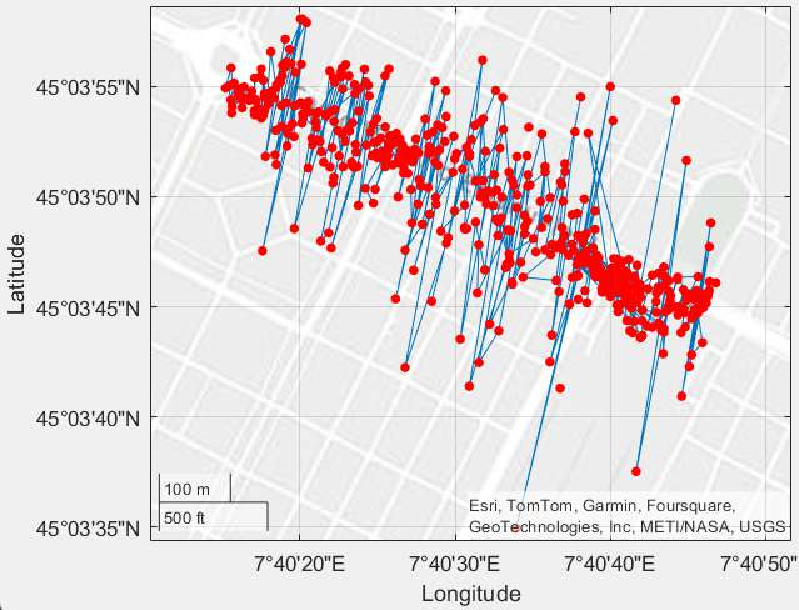
\includegraphics[width=1\linewidth]{images/C_No_filter_higher_20.pdf}
    \caption{Filter enabled}
    \label{fig:C_No_filter_higher_20}
  \end{subfigure}
  \begin{subfigure}{.22\textwidth}
  \centering
    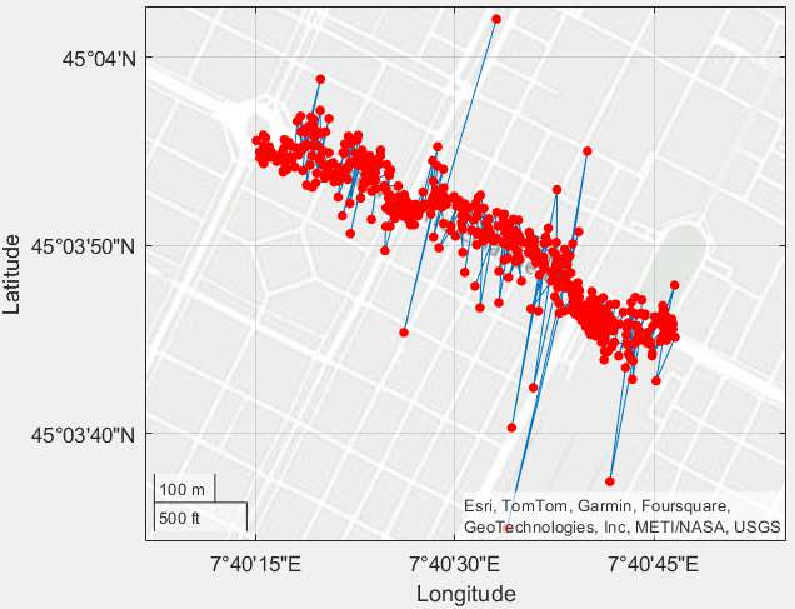
\includegraphics[width=1\linewidth]{images/C_No_filter_disabled.pdf}
    \caption{Filter disabled}
    \label{fig:C_No_filter_disabled}
  \end{subfigure}
  \vspace{10pt}
  \caption{Positioning solution on map}
  \captionsetup[subfigure]{position=below}
\end{figure}
\vspace{0.1cm}

\subsection{Constellation type}
\label{subsec:constellation_type}
This filter can be used to select specific GNSS satellite constellations. For instance, we might choose to rely only on the GPS constellation or opt to utilize multiple constellations. Here we activate only GPS and Galileo:
\begin{lstlisting}
dataFilter{end+1,1} = 'ConstellationType'; 
dataFilter{end,2}   = '(ConstellationType==1) | (ConstellationType==6)';
\end{lstlisting}
However, we found out that in all our measurements the only one working constellation is the GPS, so we used only this one. This depends on the software implementation of the GNSS Analysis MATLAB code. 